\documentclass[titlepage,landscape]{seminar}
\usepackage{url}
\usepackage{graphicx}
\usepackage[pdftex]{color}
\usepackage{hyperref}
\usepackage{epstopdf}
\usepackage{slides}

\newcommand{\frack}{\frac{1}{k}}
\newcommand{\TAMO}{\mbox{\bf\textcolor{blue}{TAMO}}}

\begin{document}

\myslide{
\begin{eqnarray*}
P({\bf n}|{\bf p},f) &\propto& \prod_{i=1}^I x_{11,i}^{n_{11,i}}
x_{12,i}^{n_{12,i}} x_{22,i}^{n_{22,i}} \\
P(p_{ik}|\pi,\theta) &\propto&
\mbox{Beta}\left(\frac{(1-\theta)}{\theta}\pi, 
                 \frac{(1-\theta)}{\theta}(1-\pi)\right) \\
\mbox{E}(p_{ik}) &=& \pi \\
\mbox{Var}(p_{ik}) &=& \pi(1-\pi)\theta
\end{eqnarray*}
}

\myslide{
\begin{center}
\begin{tabular}{cc}
\hline\hline
Wright & Weir \& Cockerham \\
\hline
$F_{IS}$ & $f$ \\
$F_{ST}$ & $\theta$ \\
\hline
\end{tabular}
\end{center}
}

\myslide{
\begin{center}
\begin{tabular}{c|ccc}
\hline\hline
Method & $F_{is}$ & $F_{st}$ \\
\hline
Direct            & 0.14 & 0.21 & 0.32 \\
Nei               & 0.31 & 0.24 & 0.47 \\
Weir \& Cockerham & 0.54 & 0.04 & 0.56 \\
Bayesian          & 0.53 (0.33, 0.70) & 0.11 (0.02, 0.22) \\
\hline
\end{tabular}
\end{center}
}

\myslide{
\begin{center}
\begin{tabular}{l|rrrr}
\hline\hline
Model & {\tt Dbar} & {\tt Dhat} & {\tt pD} & {\tt DIC} \\
\hline
Full  & 46.5 & 40.7 & 5.8 & 52.3 \\
$f=0$ & 73.0 & 67.6 & 5.3 & 73.8 \\
$\theta=0$ & 61.6 & 59.8 & 1.8 & 63.5 \\
\hline
\end{tabular}
\end{center}
}

\myslide{
\begin{eqnarray*}
\mbox{P}(i|k) &=& \frac{\mbox{P}(x_i|\gamma_k)}{\sum_k
  \mbox{P}(x_i|\gamma_k)} \\
x_i &=& \mbox{genotype of individual $i$} \\
\gamma_k &=& \mbox{genotype frequencies in population $k$}
\end{eqnarray*}
For example,
\begin{eqnarray*}
\mbox{P}((1,2,2,1,3)|(p_1, p_2, p_3, p_4, p_5)) = (p_1^2)(2p_2q_2)(2p_3q_3)(p_4^2)(q_5^2)
\end{eqnarray*}
}

\myslide{
\begin{table}
\begin{center}
\begin{tabular}{cc}
\hline\hline
K & Mean L(K) \\
\hline
2 & -2553.2 \\
3 & {\bf -2331.9} \\
4 & -2402.9 \\
5 & -2476.3 \\
\hline
\end{tabular}
\end{center}
\caption{Mean log probability of the data for $K=2,3,4,5$ in the {\it
    Berberis thunbergii\/} data}
\end{table}
}

\myslide{
\begin{figure}
\resizebox{\textwidth}{!}{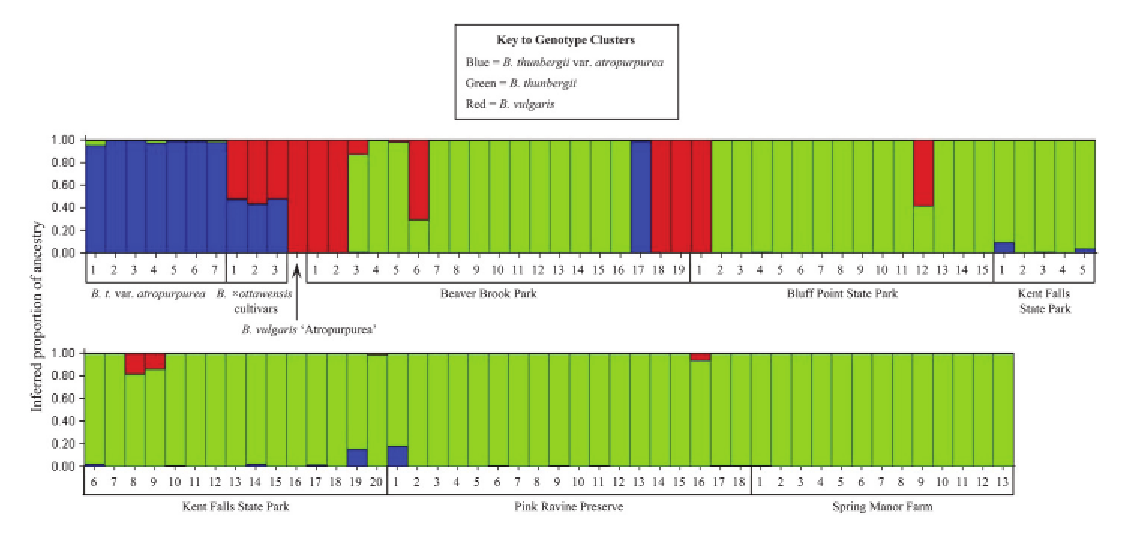
\includegraphics{lubell-structure.eps}}
\caption{Analysis of AFLP data from {\it Berberis
    thunbergii}}
\end{figure}
}

\myslide{
\begin{itemize}

\item Human Genome Diversity Cell Line Panel (HGDP-CEPH)

\item 1056 individuals, 52 geographic populations, 377 autosomal
  microsatellite loci

\end{itemize}

\begin{figure}
\resizebox{\textwidth}{!}{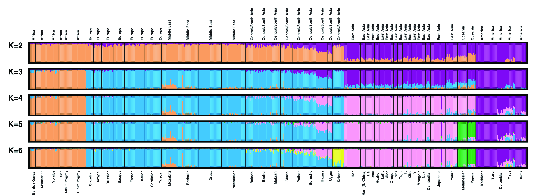
\includegraphics{HGDP-CEPH.eps}}
\end{figure}

}

\myslide{
\begin{itemize}

\item Principal components analysis of genotypes.

\item 3129 Europeans, 500,568 SNP loci

\end{itemize}

\begin{figure}
\begin{center}
\resizebox{0.5\textwidth}{!}{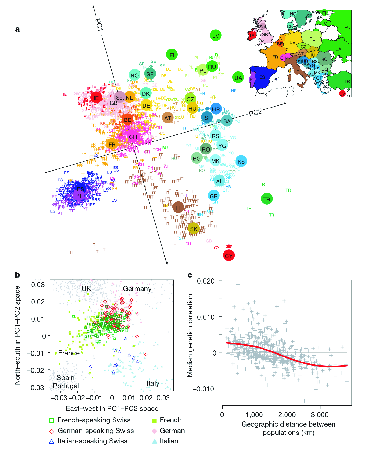
\includegraphics{human-PCA.eps}}
\end{center}
\end{figure}

}

\end{document}
